%%%%%%%%%%%%%%%%%%%%%%%%%%%%%%%%%%%%%%%%%%%%%%%%%%%%%%%%%%%%%%%%%%%%%%%%%%%%%%%%%%%%%%%%%%%%%
% 																STATE OF THE ART 																					%
%%%%%%%%%%%%%%%%%%%%%%%%%%%%%%%%%%%%%%%%%%%%%%%%%%%%%%%%%%%%%%%%%%%%%%%%%%%%%%%%%%%%%%%%%%%%%
\chapter{STATE OF THE ART}
\label{sec:stateoftheart}

The dynamic equations of kinematic chains of rigid bodies~\cite{swevers} represents the relationship between the motion of the system and the forces that cause it~\cite{craig2005introduction}. It can be considered as a mathematical model that computes forces and acceleration of the system which are relevant to the dynamics of the system. The computation of accelerations and forces based on two different algorithms can be named as forward and inverse dynamics respectively. Forward dynamics computes the accelerations based on the given joint position, velocity, torque inputs to produce the desired acceleration response in the system. It is mostly used in the simulation based systems. Whereas, inverse dynamics compute forces based on the given joint position, velocity and acceleration. These two algorithms have the system model that represents the physical properties of a system and the accuracy of the computations depend heavily on the model parameters. The algorithm that combines both the forward and inverse dynamics is referred as hybrid dynamics~\cite{featherstone2014rigid} where both the acceleration and force inputs are given to achieve a particular task. The equations of motion can be obtained through two different formulations such as the Newton-Euler and Lagrangian. Recursive Newton-Euler formulation is the most commonly used method~\cite{smits2011kdl}~\cite{featherstone2014rigid} since it is computationally efficient. The inverse dynamics computes the motion information of the rigid-body systems through the forward recursion that computes velocities and accelerations from proximal to distal links and a backward recursion is followed to compute the forces, torques from distal to proximal links. In~\cite{featherstone2014rigid}, author uses spatial vector form that combines the linear and angular aspects of motions, forces into a single six-dimensional vector and the computational efficiency increases with it. Complete dynamics of the system can be achieved by considering the uncertainties such as model errors, unmodeled dynamics~\cite{trajectorytracking_nn} which are present in the system. Model errors can be classified into kinematic and dynamic model errors but this work considers only dynamic model parameters. In~\cite{Atkeson}, author modifies the recursive Newton-Euler formulation to a linearized matrix-form for identifying the model parameters and the same method is used in the previous work~\cite{RnD2Rajagopal} where geometrical relation semantics of the rigid body are inaccurate and acceleration of the distal link that is being transmitted across joints due to the movement of the current joint is not accounted properly. In most of the rigid-body algorithms, inertial frame is attached to CoM of the rigid-body, but it is shifted to the joint origin by using the parallel-axis theorem. Re-expressing the inertia w.r.t. joint origin is essential due the unknown location of the CoM. The implementation is based on the coordinate calculations and the semantics checking is not the part of it. The numerical calculations consider the integration as an addition of two matrices but the semantics check ensures the physical meaning of those operations. The operations involved with the pose, motion and force transforms need to be semantically correct where the constraints are also applicable but the only use of numerical computations can introduce the logical errors in the system~\cite{geometicsemanticspart1}~\cite{geometicsemanticspart2}. The unknown dynamic model parameters are mass, CoM and moments of inertia and these parameters can be identified with the use of ridge regression. The kinematic chain that is created in the dynamic model based on Orocos KDL~\cite{smits2011kdl} needs correction in the frame assignments since the frame diagram in KDL is not matching with it's implementation. The friction phenomenon is one of the important effects that is present in the unmodeled dynamics. Static friction modeling has been done in the previous work~\cite{RnD2Rajagopal}. Friction modelling i.e. static friction models and the compensation~\cite{friction} techniques are discussed~\cite{corberan2012haptic}. Evolution of static friction model started with the static friction and Coulomb friction~\cite{olsson1998friction} which is the most simplified version of friction~\cite{swevers}. Then viscous friction is added with the static and Coulomb. Finally, static friction model includes the Stribeck effect along with the static and viscous friction. The model of friction that includes Stribeck friction is shown in the following figure

\begin{figure}[h]
\centering
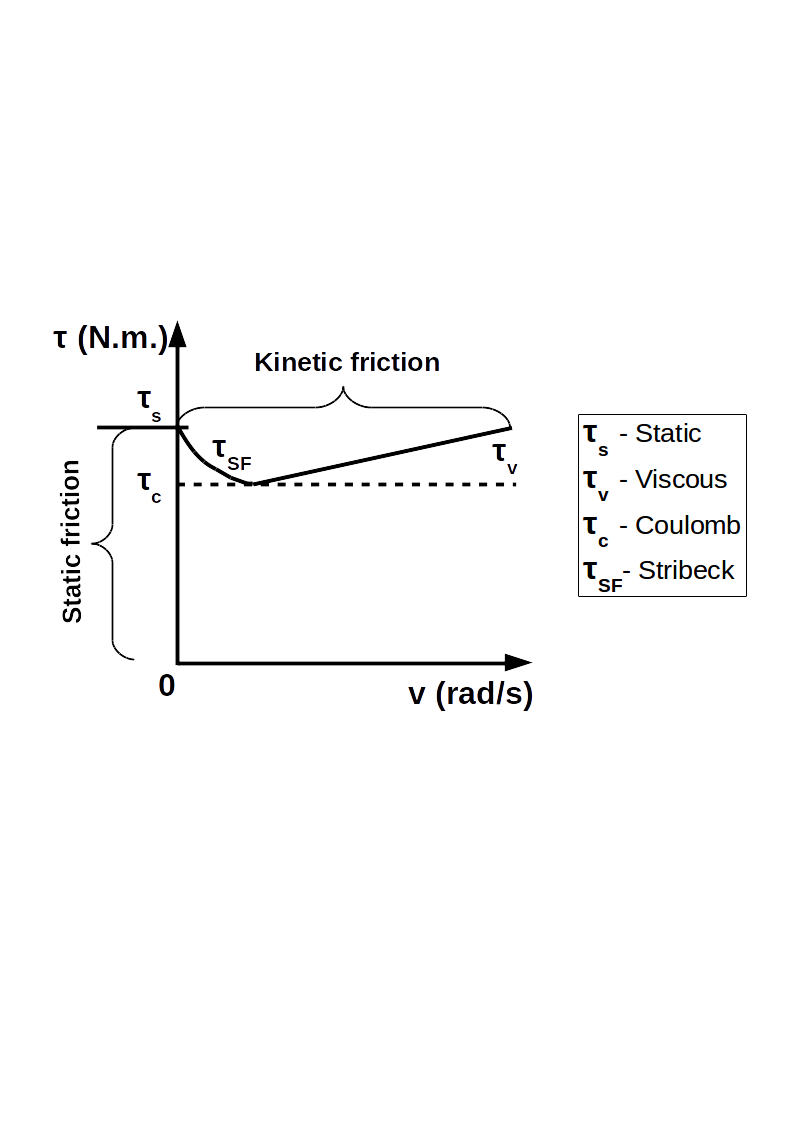
\includegraphics[width=100mm, trim=0 320 0 220]{pictures/friction_soa}
\caption{Friction model}
\end{figure}

The next important module of consideration in this work is the process control. PID controller is used by many of the standard industrial manipulators where each joint is attached with an independent PID. Mostly, single axis PID control scheme is used in the control applications~\cite{cascadedcontrol} and the controller gains can be tuned with different methods starting from empirical tuning (step-response based tuning)~\cite{astrom1995pid} to auto-tuning methods. The tracking accuracy of this method suffer in high-speed operations due the constraints in the mechanical systems. As discussed before, the manipulators are non-linear systems, it is important to account the complete dynamics of the system for the improved trajectory tracking~\cite{swevers}. There are different kinds of motion control methods available for the robot manipulators such as impedance control, computed-torque control which also has computed-torque like control~\cite{Chung2016}. Impedance control considers the interaction between the robot and the environment by accounting the dynamic characteristics of the system~\cite{de2012theory} rather than just doing force regulation based on the positions. In~\cite{muggler2013torque}, computed-torque control with the PD controller is put to work in the youBot manipulator along with dynamic model. The author has considered only the gravitational torques $\tau_g(q)$ in mathematical model and it does not account for torques due to friction. But this method needs accurate model parameters that can improve the overall result of the control scheme. It is important to consider the finding provided by the author~\cite{muggler2013torque} that the maximum applicable torque provided by the manufacturers are not sufficient to move the joints of the robot in some of the configurations of the manipulator. So, the author proposes a method that can compute the maximum applicable torque for the individual joints of the manipulator with the following equation~\eqref{eq:maxtorquemuggler}.

\begin{equation}
	\overbrace{\tau_{max}}^\text{nx1} = \overbrace{\textbf{M}_{max}}^\text{nxn} \overbrace{\textbf{K}_p}^\text{nxn} \overbrace{\textbf{e}_{max}}^\text{nx1}
\label{eq:maxtorquemuggler}
\end{equation}

where, $\tau_{max}$ represents the $n\times1$ matrix of torque that represents the maximum torque allowed in n joints of the manipulator and it is obtained by computing the product of the maximized manipulator inertia matrix, the proportional gain $K_p$ of the controller and the maximum possible joint position error $e_{max}$ and the error depends on the specifications of the particular joint. Input to the maximized manipulator inertia matrix is the joint positions where the manipulator joints are pushed to it's maximum in order to get the maximized inertia matrix. 

Chung~\cite{Chung2016} discusses computed-torque control scheme with the following formulation

\begin{equation}
\tau = H(q) \textit{v} + C(q,\dot{q})\dot{q} + \tau_g(q)
\end{equation} 

where computed torque-control consists of an inner non-linear compensation loop and the outer-loop with the control signal \textit{v}. This \textsl{control law is then substituted in the }dynamic model of the manipulator where $\ddot{q}_d$ is replaced with the control input \textit{v}. The substitution of this control law in the model solves a non-linear problem hence the linear control strategies can be applied. PD feedback control mechanism is used in the outer-loop control \textit{v}.  

\begin{equation}
\textit{v} = \ddot{q}_d + CV
\end{equation}

Computed-torque control described above is the proper control scheme and the author also provides a simple control scheme where the model and the controller works independent of each other (control input is not fed to model). Feed-forward and computed-torque control schemes discussed by~\cite{34773} results with reduction in the tracking error with the complete dynamics of the system. The model based controller requires accurate control on joint torque and it depends on the accuracy of joint position and velocity data. The computed torque-like control works by adding the variable compensation in the outer loop for accurate trajectory tracking~\cite{Chung2016} due to the uncertainties in the dynamic model. YouBot manipulator can be visualized in Simbody~\cite{sherman2011simbody} where the dynamics simulations can be achieved based on the recursive Newton-Euler formulation. Torque sensor can be created with the measured forces of gravity, bias and body forces, and it completes formulation of the generalized forces. Then the forces observed in the Cartesian space can be converted to joint torques. This library can be very useful in simulating the behaviour of the manipulator for the given motion control applications before testing it in the real robot.